\documentclass[a4paper,11pt]{report}}}

\usepackage[utf8x]{inputenc}	% lettere accentate da tastiera
\usepackage[italian]{babel}	% per scrivere in italiano
\usepackage[intlimits]{amsmath}
\usepackage{amssymb}
\usepackage{latexsym}
\usepackage{eucal} 
\usepackage{eufrak} 
\usepackage{tabularx,siunitx,booktabs,graphicx,tipa,quoting,wrapfig,multicol}

\sisetup{output-decimal-marker={,}}
\usepackage{amsthm}

\theoremstyle{plain} 
\newtheorem{thm}{Teorema}[subsection] 
\newtheorem{cor}[thm]{Corollario} 
\newtheorem{lem}[thm]{Lemma} 
\newtheorem{prop}[thm]{Proposizione}
\newtheorem{prin}[thm]{Principio} 
\newtheorem{form}[thm]{Formula}
\newtheorem{defn}{Definizione}
\newtheorem{oss}{Osservazione} 


\newcommand{\f}{\text{f}}
\newcommand{\g}{\text{g}}
\title {
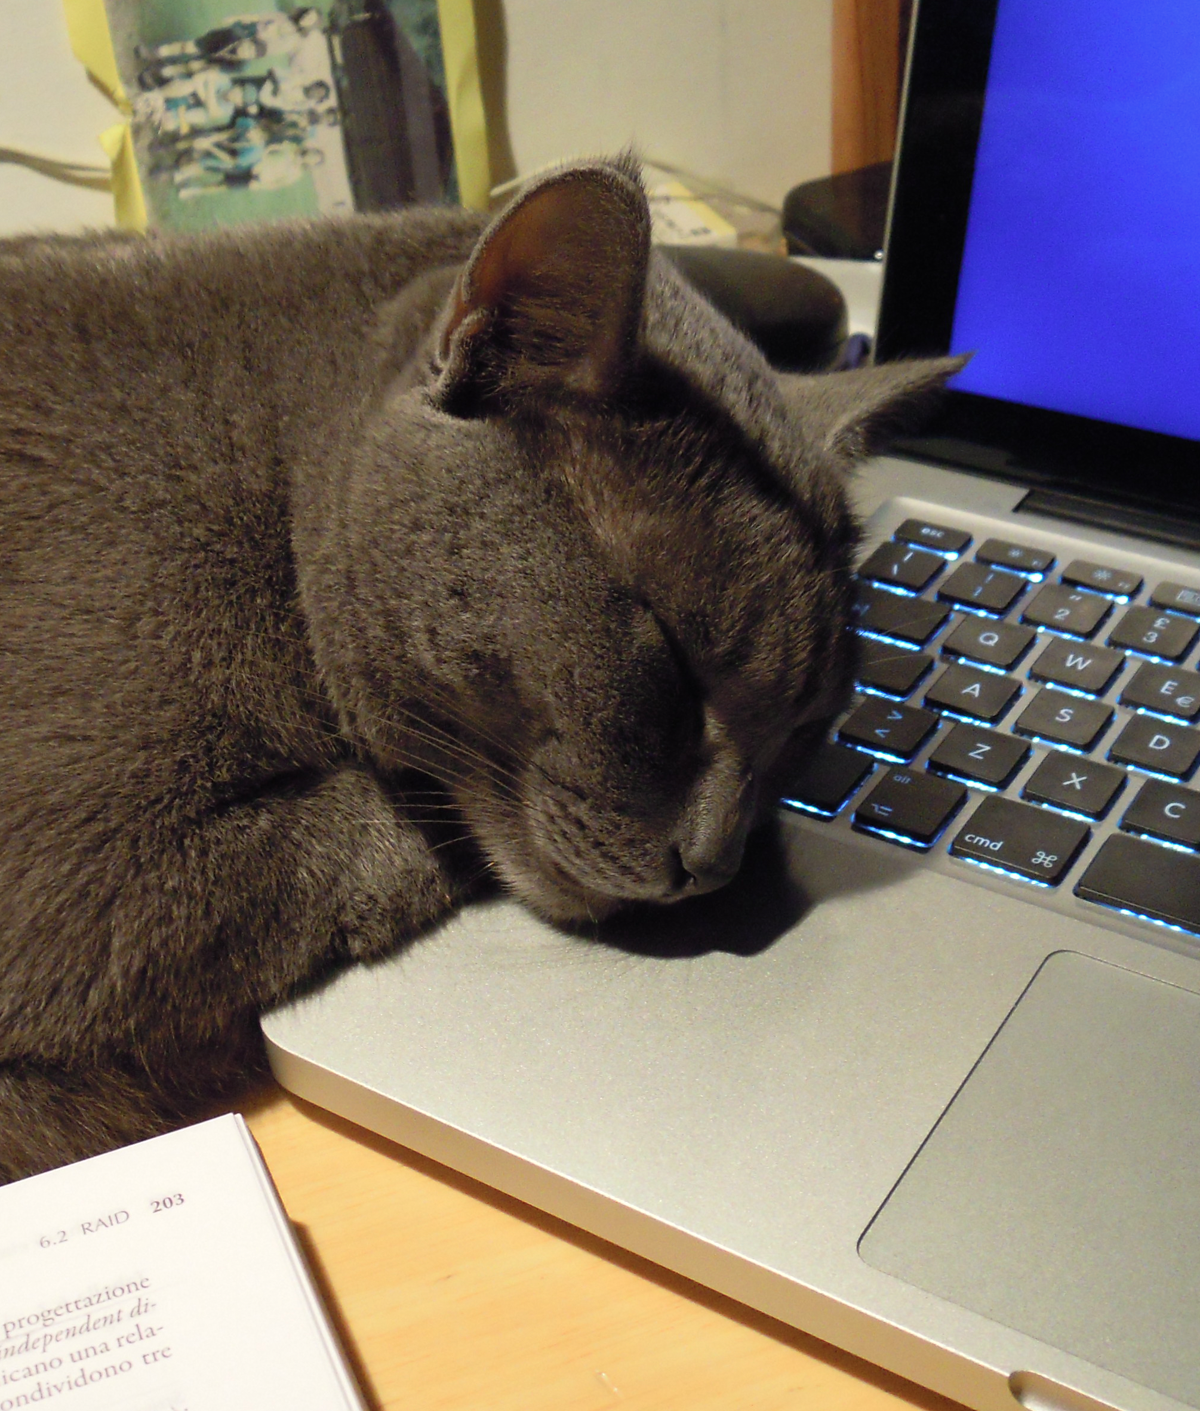
\includegraphics[scale=1]{Copertina}\\
Appunti del corso di Calcolo\\ {\large per ripetere un po'}}
\author{Matteo Scarpa}


\begin{document}

\maketitle

\thanks{
 \begin{center}
Appunti del corso di
 Analisi fatto da Matteo Scarpa a titolo gratuito prendendo dalle dispense del professor Antonio Grioli e dagli appunti presi in classe per cui soggetti ad \textit{errori e orrori}. Visto che il programma è lo stesso è adatto anche per il corso di Calcolo di Ca'Foscari.
  È presente anche su Google~Drive per problemi di "stabilità" di Dropbox.\\
  Il lavoro verra ampliato durante la durata del corso pertanto \textbf{sconsiglio di stamparlo} perchè è in continuo aggiornamento.
  È stato scelto il formato pdf perchè universale. In caso di errori segnalarli a \textit{mscarpa@dsi.uvine.it}\\ o mandarmi un mp.
 Si ringrazia Ceasar per il sostegno e le correzioni e PiGreco (il gatto in copertina) per i momenti di distrazione.
\end{center}
}

 \tableofcontents
 \newpage

\section{Dato per scontato\\ anche se mai imparato}
Questa sezione è dedicata a chi ha bisogno di un ripasso di elementi non spiegati nel corso ma comunque necessari per gli argomenti del corso.
\subsection{Disequazioni}
 Queste sono le formule per dire quando $y=ax^2+bx+c$ con $a>0$ è positivo. Le formule per $a<0$ si ricavano moltiplicando per $-1$ le sequenti formule:
 
 \begin{gather*}
 \Delta>0 \quad \f (x)\quad x<x'\quad \cup x>x''\\
 \Delta=0 \quad \forall x \in \text{Dominio}\\
 \Delta>0 \quad \forall x \in \text{Dominio}\\
 \end{gather*}

\begin{wrapfloat}{figure}{r}{0pt}
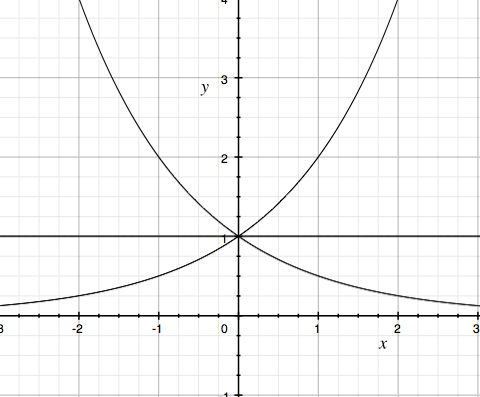
\includegraphics[width=0.5\columnwidth]{Esponenziale}
\caption{Funzioni esponenziali con $a>1$, $a=1$ e $a<1$}
\end{wrapfloat}

\subsection{Esponenziale e logaritmi}

Si può vedere dalla figura che $a^x$ è decrescente se $0<a<1$ ed è crescente se $a>1$. Se $a=1$ il grafico è quello della retta $y=1$.
La funzione esponenziale \f$:x\to a^x$ è monotona quindi invertibile. Infatti la sua inversa è la funzione logaritmo in base a di x e si indica con \f$^-1 :x \to \lg_a x$.
Il logaritmo in base a di x è l'esponente di a che serve per ottenere x.\\
 \newline
 \paragraph{NB:}
  \begin{gather}
   {\lg}_a 1=0\\
   {\lg}_a a=1\\
   {\lg}_a (xy)= {\lg}_a x + {\lg}_a y\\
   {\lg}_a (\frac{x}{y}={\lg}_a x - {\lg}_a y\\
   {\lg}_b x=\frac{{\lg}_a x}{{\lg}_a b}
  \end{gather}

 \subsection{Trigonometria}
\begin{wrapfloat}{figure}{r}{0pt}
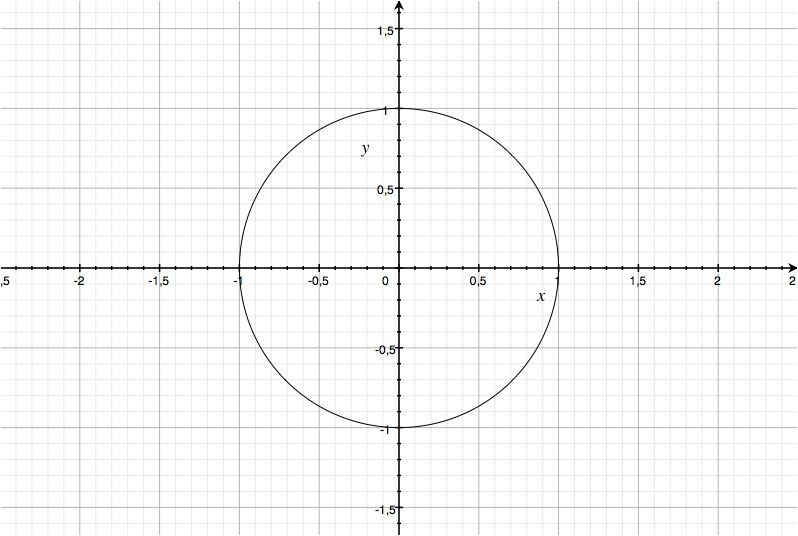
\includegraphics[width=0.5\columnwidth]{Trigonometria}
\caption{Circolo goniometrico}
\end{wrapfloat}
La trigonometria si basa tutto sul circolo goniometrico, circonferenza di raggio unitario (fig 1.2) su cui si disegnano gli angoli con cui si lavora.
La trigonometria usa come misura degli angoli i \textit{radianti} ovvero la misura dell'angolo che sottende un arco di circonferenza uguale al raggio. Per convertire dai gradi basta ricorrere alla seguente proporzione:
\[
\text{gradi}:360=\text{radianti}:2\pi
\]

La tabella mostra~gli angoli notevoli in gradi e radianti.\\

\[\begin{array}{cc}
\toprule
Gradi   & Radianti \\
\midrule
30 & \frac{\pi}{6} \\
60 & \frac{\pi}{3} \\
45 & \frac{\pi}{4} \\
90 & \frac{\pi}{2} \\
180 & \pi \\
270 & \frac{3}{2}\pi \\
360 & 2\pi \\
\bottomrule
\end{array}\]
 

 \paragraph{Seno e Coseno}
 Dato l'angolo orientato $\alpha=\widehat {aop}$ si definiscono $\sin$ e $\cos$ di $\alpha$ rispettivamente come l'ordinata y e l'ascissa x del punto~$\mathbb{P}$:
 \[
 \sin \alpha =yp
 \text{ e }
 \cos \alpha =xp
 \]
 
\paragraph{NB:}
 \begin{gather}
    \sin(\frac{\pi}{2})-\alpha=\cos\alpha\\
    \cos(\frac{\pi}{2}-\alpha)=\sin\alpha\\
    \sin(\frac{\pi}{2}+\alpha)=\cos\alpha\\
    \cos(\frac{\pi}{2}+\alpha)=-\sin\alpha\\
    \sin(\pi-\alpha)=\sin\alpha\\
    \cos(\pi-\alpha)=-\cos\alpha
 \end{gather}
 
 Altre formule utili della trigonometria:
 
 \begin{form}[Ugualianza fondamentale]
 \[
 \sin^2(\alpha)+\cos^2(\alpha)=1
 \]
 \end{form}
 
 \begin{form}[Addizione-sottrazione seno]
 \[
 sen(x\pm y)=\sin x \cos y\pm\cos x \sin y
 \]
 \end{form}
 
 \begin{form}[Addizione-sottazione coseno]
 \[
 \cos(x\pm y)=\cos x\cos y\pm\sin x \sin y
 \]
 \end{form}
 
 \begin{form}[Duplicazione seno]
	\[
	\sin 2x=2\sin x\cos x
	\]
 \end{form}
 
 \begin{form}[Duplicazione coseno] 
\[
\cos^2 x-\sin^2 x
\]
 \end{form}
 
 \begin{form}[Prostaferesi seno]
 \[
 \sin x \pm \sin y=2\sin(\frac{x\pm y}{2}) \cos(\frac{x \pm y}{2})
 \]
 \end{form}

 \begin{form}[Prostaferesi coseno]
 \[
 \cos x +\cos y=+2\cos(\frac{x+y}{2})\cos(\frac{x-y}{2})
 \qquad
 \cos x -\cos y=-2\sin(\frac{x+y}{2})\sin(\frac{x-y}{2})
 \]
 \end{form}
 
 \paragraph{Tangente}
 La \textit{tangente} non è altro che $\frac{\sin x}{\cos x}= \tan x$. Le formule riportate qui sopra permettono di ricavare le formule equivalenti per la funzione tangente.
 
 \paragraph{Altre funzioni trigonometriche}
 Sono \textit{secante, cosecante} e \textit{cotangente}.  Esse sono delle funzioni derivate da quelle viste fin ora:\\
\begin{gather}
 \sec x=\frac{1}{\cos x}\\
 \cos x=\frac{1}{\sin x}\\
 \cot x=\frac{1}{\tan x}\\
\end{gather} 



\section{Cenni di insiemistica}
\textbf{Le nozioni di insieme di elementi di un insieme e di appartenenza vanno assunte come nozioni primitive.}\\

\subsection{Notazioni}
	\begin{math}
	 a\in A
	\end{math}
 Significa che è un elemento dell'insieme A\\
	\begin{math}
	 a\notin A
	\end{math}
 Significa che non è un elemento dell'insieme A\\
 Un insieme può essere definito espicitamente elencandone tutti i suoi elementi (ovviamente solo se è un insieme finito, cioè formato da un numero finito di elementi) oppure dando una legge oggettiva che permetta di identificare in maniera certa tutti i suoi elementi.
 
 \paragraph{Esempi}
 	\begin{math}
 	 A=\left\{{1,3,7}\right\}
 	\end{math}
 Rappresenta l'insieme i cui elementi sono i numeri 1,3,7\\
\begin{math}
 	 A=\left\{{2,4,6,8,10}\right\}
 	\end{math}
 Rappresenta l'insieme i cui elementi sono i numeri 2,4,6,8,10. Tale insieme potrebbe essere individuato in altro modo in base alla\\
 seguente legge:\\
\textit{ A è l'insieme formato da i numeri pari positivi minori o uguali a 10}\\
 	\begin{math}
 	 A=\left\{{\forall n \in N| n\geq100}\right\}
 	\end{math} 
 Si legge:\\
 \textit{ A è l'insieme di tutti i numeri interi (come vedremo più avanti l'insieme dei numeri naturali si indica con $\mathcal{N}$})\\
 
\subsection{Insiemi}

\paragraph{Sottoinsiemi impropri o sottoinsiemi}
 L'insieme A si dice sottoinsieme di B (e si scrive $A\subseteq B$) se ogni elemento di A è anche elemento di B.
 
\paragraph{Sottoinsiemi Propri}
 A si dice sottoinsieme proprio di B (e si scrive $A \subset B$) se ogni elemento di A appartiene a B e inoltre vi è almeno un elemento di B che non appartiene ad A\\

 \subsection{Operazioni sugli insiemi}

 \paragraph{Unione}
 Dati due insiemi A e B si definisce la loro unione (che si scrive $C=A \cup B$) l'insieme C formato da tutti gli elementi di A e da tutti gli elenemti di B (copiati una sola volta anche se presenti sia in A che in B).

 \paragraph{Esempio}
  \[
   A=\left\{{2,-5,4}\right\} B=\left\{{0,3,-5}\right\}\Rightarrow A\cup B=\left\{{2,-5,4,0,3}\right\}
  \]
  In maniera ovvia le operazioni di unione e di intersezione possono estendersi ad un numero qualsiasi di insiemi.

 \paragraph{Complemento di A in B}
  Si indica con $B/A$ ed è definito come l'insieme di tutti gli elementi di B che non appartengono ad A.

  \paragraph{Esempio}
  Riferendosi agli esempi precedenti si ha:
  \begin{math}
  B/A=\left\{{0,3}\right\}
  A/B=\left\{{2,4}\right\}
  \end{math}

 \paragraph{Proprietà delle operazioni sugli insiemi}
 \begin{gather*}
  A\cup B=B\cup A\\
  A\cup(B\cup C)=(A\cup B)\cup C\\
  A\cap B=B \cap A\\
  A\cap (B\cap C)=(A\cap B)\cap C\\
  A\cap (B\cup C)=(A\cup B)\cap (A\cup C)\\
  A\cup (B\cap C)=(A\cap B)\cup (A\cap C)\\
  C/ A\cup B=(C/A)\cap (C/B)\\
  C/ A\cap B=(C/A)\cup (C/B)\\ 
 \end{gather*}
 Due insiemi si dicono uguali se contengono gli stessi elementi. In tal caso valgono contemporaneamente
 	$A \subseteq B$
 	e
 	$A \supseteq B$\\
L'insieme che non contiene alcun elemento si chiama insieme vuoto $\phi$
Due insiemisi dicono disgiunti se la loro intersezione è l'insieme vuoto, cioè se:
\[
A\cap B=\phi
\]
Valgono le seguenti proprietà:
\begin{gather*}
	A\cup \phi=A \quad
	A\cap \phi=\phi \quad
	A/ \phi=A
 \end{gather*}

\paragraph{Prodotto Cartesiano}
Dati due insiemi A e B chiamasi prodotto cartesiano (e si indica con AxB) l'insieme delle coppie ordinate (a,b) con $a\in A$ e $b\in B$

\paragraph{Insiemi numerici}

 \paragraph{I numeri naturali $\mathbb{N}$}
  L'insieme $\mathbb{N}$ indica l'insieme dei numeri naturali. È chiuso rispetto alla somma e al prodotto; questo vuole dire che il risultato di una somma o di un prodotto è sempre in $\mathbb{N}$.

 \paragraph{I numeri interi con segno $\mathbb{Z}$}
  L'insieme $\mathbb{Z}$ indica l'insieme dei numeri interi relativi con segno. È chiuso per le operazioni di somma, prodotto e sottrazione.

  \paragraph{Insieme dei numeri razionali $\mathbb{Q}$}
  L'insieme $\mathbb{Q}$ indica l'insieme dei numeri razionali. È chiso rispetto somma, prodotto, sottrazione e divisione diversa da 0. I suoi numeri possono essere rappresentati come coppie di numeri interi in cui il primo è il numeratore e il secondo è il denominatore~$(n,d)$. Due numeri razionali $\frac{a}{b}$ e $\frac{a'}{b'}$ sono equivalenti solo se $ab'=a'b$. I numeri razionali possono anche rappresentare decimali finiti o periodici quali 
  $\frac{2}{3}=0, \overset {\scriptscriptstyle-}{6} $ oppure
  $\frac{3}{4}=0,75 $

 \paragraph{Insieme dei numeri reali $\mathbb{R}$}
 L'insieme $\mathbb{R}$ indica l'insieme dei numeri reali. Può essere espresso attraverso il concetto di limite o con il concetto di elemento di separazione di due classi contigue di numeri razionali.\\
 Per esempio $\sqrt[2]{2}$ può essere l'elemento di separazione fra la classe formata da tutti i numeri negativi, lo zero e tutti i numeri positiviil cui quadrato è pari o superiore a 2 e la classe formata da tutti i numeri il cui quadrato è superiore a 2.In oltre gode della proprietà di completezza ovvero che:
 \[
 a \leq \delta \leq b \quad \forall a \in A \quad \wedge \forall b \in B
 \]
 


\section{Limiti}
 
 \subsection{Nozioni legate ai limiti}
  
  \paragraph{Estremo superiore e inferiore}
  	In un insieme completo l'estremo superiore si definisce:
  	 \begin{quote}
  	  Dato un insieme $A \subset \mathbb{R}$ chiamasi maggiorante ogni numero $k\geq a$ $\forall a \in A$.
  	 \end{quote}
	In tal caso si dice limitato superiormente e viene chiamato \textit{estremo~superiore} il più piccolo dei suoi maggioranti. Se tale numero $\delta \in A$ si dice \textit{massimo di A}, altrimenti si definisce soltanto come estremo superiore di A.\\ Nel caso che A non ammetta maggioranti allora è \textit{illimitato superiormente} e il suo estremo è $+\infty$. Analogamente si definisce \textit{estremo inferiore}.
	
	\paragraph{Palla aperta di centro P0 e raggio $\delta$}
	LA si indica con $\mathbb{B}(P0,\delta)$ ed è data dai punti
	$P\in \mathbb{R}|d(P,P0)<\delta$.\\ A questo punto risulta evidente che i concetti e le definizioni date in $\mathbb{R}^{2}$ e $\mathbb{R}^{3}$ possono estendersi a uno spazio cartesiano $\mathbb{R}^{n}$ qualsiasi.
	
	\paragraph{Spazi metrici}
	 \begin{quote}
	  Un insieme $\mathbb{X}$ è detto spazio metrico e i suoi elementi vengono chiamati punti se esiste una funzione 
	  \textit{$d:\mathbb{X}x\mathbb{X}\to \mathbb{R}^{+}$} che chiameremo \textit{distanza} tale che:
	  \begin{gather}
	   d(x,y)\geq 0 \quad \forall x,y \in \mathbb{X}\\
	   d(x,y)=0 \quad \Leftrightarrow x=y\\
	   d(x,y)\leq d(x,y)+d(y,z) \quad \forall x,y,z\in \mathbb{X}
	  \end{gather}
	 \end{quote}
	
	\subsubsection{Definizioni legate agli spazi metrici}
     
     \paragraph{Intorno sferico}
      Chiamasi \textit{intorno sferico} o \textit{palla aperta} di centro x0$\in \mathbb{X}$ e raggio $\delta >0$, l'insieme dei punti $x\in \mathbb{X}$ tali che: $d(x_0,x)<\delta$\\
      
      \paragraph{Intorno}
      Chiamasi \textit{intorno} di $x_0$ qualsiasi sottoinsieme $\mathbb{H} \subseteq \mathbb{X}$ contenente un intorno sferico di $x_0$
      
      \paragraph{Aperto}
      Un sottoinsieme $\mathbb{A}\subseteq \mathbb{X}$ si dice \textit{aperto} se ogni suo punto è centro di un intorno sferico tutto contenuto in $\mathbb{A}$
      
      \paragraph{Chiuso}
      Un sottoinsieme $\mathbb{B}\subset \mathbb{X}$ si dice \textit{chiuso} se il suo complemento in x x/$\mathbb{B}$ è aperto.
      \textbf{N.B.}: l'intero spazio $\mathbb{X}$ e l'insieme vuoto $\phi$ sono gli unici due insiemi sia aperti che chiusi.
     
     \paragraph{Punto di frontiera}
      Un punto $x_0$ si dice di \textit{frontiera} per $\mathbb{A} \subseteq \mathbb{X}$ se in ogni suo interno sferico cadono sia punti si $\mathbb{A}$ che punti di $\mathbb{X}/\mathbb{A}$. Il punto $x_0$ può appartenere ad $\mathbb{A}$ oppure ad $\mathbb{X}/\mathbb{A}$.
     
     \paragraph{Punto di accumulazione}
      Un punto $x-0$ si dice di \textit{accumulazione} per $\mathbb{A}$ se in ogni suo intorno cadono punti di $\mathbb{A}$ diversi da $x-0$. Anche in questo caso $x-0$ può appartenere sia ad $\mathbb{A}$ che ad $\mathbb{X}/\mathbb{A}$.
      
     \paragraph{Punto isolato}
     Un punto $x_0$ si dice \textit{isolato} se esiste una palla aperta con centro in $x_0$ che non contiene altri punti di $\mathbb{A}$
     
     \subsubsection{Funzioni}
     
     \paragraph{Crescenti}
      \f{} si dice \textit{crescente} se:
      \[ 
      x'' > x' \to \f(x'')>\f(x')
      \]
      
      \paragraph{Decrescenti}
      \f{} si dice \textit{decrescente} se:
      \[
      x'' > x' \to \f(x'')<\f(x')
      \]
      
      \paragraph{Monotone}
      È evidente che le funzioni strettamente monotone sono iniettive e quindi invertibili.
      
      \paragraph{Periodiche}
      Una funzione \f{} di $\mathbb{R}$ in $\mathbb{R}$ si dice \textit{periodica} se esiste almeno un numero reale $\alpha >0$ tale che:
      \[
      \f(x \pm n \alpha)=\f(x) \quad \forall x \in \mathbb{R} \wedge \forall n \in \mathbb{N}
      \]
      
      \paragraph{Continue}
      Una funzione si dice continua nel punto $x0\in$ Dominio \f() se:
      \[
      	\mathop{\lim}\limits_{x \to x_0}\text(\f)(x)=\text{\f}(x)
      \]
      
      Si dice continua su tutto il dominio se vale $\forall x_0\in\text{Dominio}\f()$. 
      L'insieme delle funzioni continue nell'insieme D si indica con il simbolo $C^0(D)$
      
      \subsection{Limite a variabile singola}
      
       \paragraph{Definizione:}
        Sia \f$(x)$ una funzione definita attorno al punto x0 (non necessariamente anche nel punto) si dirà che:
        \[
        \mathop{\lim}\limits_{x \to x_0} \f (x)= L
        \]
        Se $ \forall \varepsilon >0$ piccolo a piacere esiste in corrispondenza un intorno H di $x_0$ per~cui:\\
        \[
        \left|{\text{\f}(x)-L}\right|<\varepsilon \text{ per } x\in H/x_0
        \]
        si chiama 
        
        \begin{gather*}
        \mathop{\lim}\limits_{x \to x_0^+} \text{\f} (x)=L\\
        \text{\textit{limite destro}}\\
        \mathop{\lim}\limits_{x \to x_0} \f (x)= L
        \end{gather*}
        
        Se $ \forall \varepsilon >0$ piccolo a piacere esiste in corrispondenza un intorno H di x0 per~cui:
        \begin{gather*}
        \left|{\text{\f}(x)-L}\right|<\varepsilon \text{ per } x\in H/x_0\\
        \text{si chiama}\\
        \mathop{\lim}\limits_{x \to x0^-} \text{\f} (x)=L 
        \text{\textit{limite sinistro}}
        \end{gather*}
		
		\subsubsection{Teoremi dei limiti}
		 \begin{thm}[Teorema dell'unicità del limite:]
		 \textbf{}\\
		  Se esiste $\mathop{\lim}\limits_{x \to x_0}\f(x)\to x_0$ questo è unico. Ne seque che la condizione necessaria e sufficente affinche esista $\mathop{\lim}\limits_{x \to x_0}\f(x)$ è che in $x_0$ esistano il limite destro e sinistro e che siano uguali tra loro.\\
		 \end{thm}
		 
		Dati i limiti\\ 
		\[
		 \mathop{\lim}\limits_{x \to x_0}\f (x)=L1\quad
		 \mathop{\lim}\limits_{x \to x_0}\g (x)=L2
		\]
		  sono dimostrabili i seguenti teoremi:
		  
		 \begin{thm}[Limite della somma e della differenza:]
			\[
		  \mathop{\lim}\limits_{x \to x_0}[\f(x)\pm \g (x)]=L1\pm L2
		  \] 
		 \end{thm}
		 
		  \begin{thm}[Limite del prodotto:]
		  \[
		  \mathop{\lim}\limits_{x \to x_0}[\f(x)\g(x)=L1*L2
		  \]
		  \end{thm}
		  
		  \begin{prin}[Di sostituzione:]
		  Se \f(x) e g(x) sono \textit{infinitesimi di ordine superiore} o \text{infiniti di ordine inferiore} di ${\f}_1(x)$ e ${\g}_1(x)$ allora si ha:
		  \[
		  \mathop{\lim}\limits_{x \to x_0}\frac{\text{\f(x)}\pm \text{\f}_1(x)}{\text{g(x)}\pm \text{g}_1(x}
		  \]
		  \end{prin}

		  
		  \begin{thm}[Limite del quoziente:]
		  \[
		  \mathop{\lim}\limits_{x \to x_0}\frac{ \text{\f}(x)} {\text
		  {g}(x)}=\frac{L1}{L2}
		  \]
		  \end{thm}
		  
		  \begin{thm}[Limite del rapporto di due polinomi:]
		  \begin{gather*}
		  \mathop{\lim}\limits_{x \to \infty}\frac{a_nx^n+a_{n-1}x^{n-1}+…+a_1x+a_0}{b_mx^m+b_{m-1}x^{m-1}+…+b_1x+b_0}\text{ con }a_n\ne 0 \and b_m\ne 0\text{ è:}\\ 
		  \infty\text{ se }n>m\\
		  \frac{a^n}{b^m}\text{ sse }n=m\\
		  0\text{ se }n<m\\
		 \end{gather*}
		 \end{thm}

\begin{thm}[Limite di una funzione composta da due funzioni continue:]
		  \[
		  \mathop{\lim}\limits_{x \to x_0}\text{\f}\left[{g(x)}\right]=\text{\f}(l)
		  \]
		  \end{thm}
		  
		 I teoremi qui enunciati valgono sempre a meno che non si presenti uno dei seguenti casi indeterminati:
		 
		\begin{gather*}
		  \pm\infty\mp\infty\qquad \infty *0\qquad
		  \frac{0}{0}\qquad
		  1^{\infty} \qquad
		  \frac{\infty}{\infty}
		 \end{gather*}
		  
		  \subsubsection{Infinitesimi e infiniti}
		   La funzione $\mathop{\lim}\limits_{x \to x_0} \text{\f}(x)=0$ si dice \textit{infinitesima} in $x_0$ o in $\infty$.\\
		   La funzione $\mathop{\lim}\limits_{x \to x_0} \text{\f}(x)=\infty$ si dice \textit{infinita} in $x_0$ o in $\infty$.\\
		   
		   Date due funzioni \f(x) e g(x) infinitesime si dice che \f(x) è \textit{infinitesima di ordine superiore} rispetto a g(x) se
		   \[
		   \mathop{\lim}\limits_{x \to x_0}\frac{\text{\f(x)}}{g(x)}=0
		   \]
		   Date due funzioni \f(x) e g(x) infinite si dice che \f(x) è \textit{infinita di ordine superiore} rispetto a g(x) se
		   \[
		   \mathop{\lim}\limits_{x \to x_0}\frac{\text{\f(x)}}{g(x)}=\infty
		   \]
		   
		   \subsubsection{Limiti notevoli o particolarmente importanti}
Mi permetto di aggiungere dei limiti oltre ai limiti notevoli o variazioni di essi per semplificare il lavoro con i limiti in quanto i seguenti sei limiti sono i limiti indefiniti più comuni.
		   \begin{gather}
		   \mathop{\lim}\limits_{x \to 0} \frac{\mathbb{e}^x-1}{x}=1\\
			\mathop{\lim}\limits_{x \to \infty} \left({1+\frac{1}{x}}\right)^x=e\mathbb{e}\\
		   \mathop{\lim}\limits_{\text{\f}(x) \to 0}\frac{\sin\text{\f}(x)}{\text{\f}(x)}=1\\
			\mathop{\lim}\limits_{x \to 0}\frac{1-\cos(x)}{x}=0\\
			\mathop{\lim}\limits_{x \to 0}\frac{1-\cos(x)}{x^2}=\frac{1}{2}\\
			\mathop{\lim}\limits_{x \to 0}\frac{\log(1+x)}{x}=1
			\end{gather}

\section{Derivate}

\subsection{Derivata a una variabile}
	La \textit{derivata} non è altro che un limite. Infatti la derivata è il limite del rapporto incrementale della funzione \f.
\[{\rm d}\text{\f}(x)=\mathop{\lim}\limits_{h \to 0} \frac{\text{\f}(x_0+h)-\text{\f}(x_0)}{h}
\]	
	\subsubsection{Tabella delle derivate fondamentali e non}
	\begin{gather*}
		 {\rm d}(k)=0\\
		 {\rm d}(x)=1\\
		 {\rm d}(x^n)=nx^{n-1}\\
		 {\rm d}(\left|{x}\right| )=\frac{\left|{x}\right|}{x} \text{ oppure }\frac{x}{\left|{x}\right|}\\
		 {\rm d}(A^x)=A^x\log{A}\\
		 {\rm d}\sqrt[2]{x}=\frac{1}{2\sqrt[2]{x}}\\
		 {\rm d}(\log_a{x})=\frac{1}{x}\log_a{e}\\
		 {\rm d}(e^x)=e^x\\
		 {\rm d}(\sin{x})=\cos{x}\\
		 {\rm d}(\cos{x})=- \sin{x}\\
		 {\rm d}(\tan{x})=\frac{1}{\cos^2{x}} \text{ o } i+\tan'2x\\
		 {\rm d}(\arctan{x})=\frac{1}{1+x^2}\\
		 {\rm d}\frac{1}{x}=-\frac{1}{x^2}\\
		 {\rm d}(k\text{\f}(x))=k\text{\f}'(x)\\
		 {\rm d}(\arcsin x)=\frac{1}{\sqrt[2]{1-x^2}}\\
		 {\rm d}(\arccos x)=-\frac{1}{\sqrt[2]{1-x^2}}\\	\end{gather*}
	
		\subsubsection{Teoremi delle derivate}
		
		 \begin{thm}[]
		  \[
		  {\rm d}\left({\text{\f}(x)\pm g(x)}\right)=\text{\f}'(x)\pm g'(x)
		  \]
		  \end{thm}
		  
		  \begin{thm}[]
		  \[
		  {\rm d}\left({\text{\f}(x) g(x)}\right)=\text{\f}'(x) g(x)+\text{\f}(x)g'(x))
		  \]
		  \end{thm}
		  
		  \begin{thm}[]
		  \[
		  {\rm d}(\frac{\text{\f}(x)}{g(x)})=\frac{\text{\f}'(x)g(x)-\text{\f}(x)g'(x)}{g^2(x)}
		  \]
		  \end{thm}
		  
		  \begin{thm}[]
		  \[
		  {\rm d}\text{ \f}(g(x))=\text{\f}'(g(x))g'(x)
		  \]
		  \end{thm}
		  
		  \begin{thm}[]
		  \[
		  {\rm d}(\text{\f}'(x))=\frac{1}{\text{\f}'(\text{\f}^-1()x)}
		  \]
		  \end{thm}
		  
		  \begin{thm}[]
		  \[
		  {\rm d}(\text{\f}(x)^{g(x)})=\text{\f}(x)^{g(x)}\left({g'(x)\ln\left({\text{\f}(x)}\right)+\frac{g(x)\text{\f}'(x)}{\text{\f}(x)}}\right)
		  \]
		  \end{thm}
		 	
		 	\begin{thm}[Rolle]
		  Sia $\f(x)\in c'[a,b]\text{ con \f}(a)=\text{\f}(b)$ e derivabile in $]a,b[$.\\ Allora esiste almeno un punto interno ad [a,b] in cui $\f '(c)=0$
		  
		  \end{thm}
		 	
		 	\begin{thm}[Lagrange]
		   Sia $\f(x)\in c'[a,b]$ e derivabile in $]a,b[$.\\ Allora esiste almeno un punto c interno ad $[a,b]$ in cui:
		   $\f'(c)=\frac{\text{\f}(b)-\text{\f}(a)}{b-a}$
		  \end{thm}
		  
		  	\begin{cor}[Lagrange 1]
		   Sia $\f(x)\in c'[a,b]$ e derivabile in $]a,b[$.\\ Allora esiste almeno un punto c interno ad $[a,b]$ in cui:
		   $\f'(x)=0$
		  \end{cor}

		  \begin{cor}[Lagrange 2]
		  Sia $\f(x)$ e g(x) continue in $[a,b]$ e $\f'(x)=\g'(x)$ in $]a,b[$.\\ Allora $\f(x)-g(x)=k \text{ in }[a,b]$
		  \end{cor}
		  
		  \begin{cor}[Lagrange 3]
		   Sia $\f(x)\in c'[a,b]$ e derivabile in $]a,b[$.\\ Allora se $\f'(x)>0$ la funzione è crescente.\\ Se $\f'(x)<0$ la funzione è decrescente.
		  \end{cor}
		  
\subsubsection{Differenziale}

Per h=1 si ottiene:
\[
\text{\f}(x_0)+\text{\f}'(x_0)(x-x_0)=\text{\f}(x_0)+f'(x_0)\delta x
\]
per cui in una prima approssimazione si ha, in un intorno di $x_0$:
\[
\f(x)\cong \text{\f}(x_0)+\text{\f}'(x_0)\delta x
\]

da cui segue:
\[
\delta \text{\f}(x)=\text{\f}(x)+\text{\f}'(x_0)\cong \text{\f}'(x_0)\delta x
\]
La quantità $\f'(x_0)\delta x$ si chiama \textit{differenziale} di $\f(x)$ nel punto x. E si scrive:
\[
d\text{\f}(x_0)=\text{\f}'(x_0)\delta x
\]

\subsection{Derivate a più variabili}
È possibile fare una derivata a più variabili. Essa si scrive
\[
\text{\f}_y(x,y)=\mathop{\lim}\limits_{h \to 0} \frac{\text{\f}(x,y+h)-\text{\f}(x,y)}{h}
\]
e si indica
\[
\frac{{\rm d}\text{\f}}{{\rm d}x}\text{ e }\frac{{\rm d}\text{\f}}{{\rm d}y}
\]
Da questo si ricava che

\begin{gather*}
\frac{{\rm d}\f}{{\rm d}i}(x,y)=
{\f}_x(x,y)\text{ che ha u}=\left({
\begin{array}{c}
  {1}  \\
  {0}  \\
\end{array}
}\right)\\
\frac{{\rm d}\text{\f}}{{\rm d}i}(x,y)=\text{\f}_x(x,y)\text{ che ha u}
=\left({
\begin{array}{c}
  {0}  \\
  {1}  \\
\end{array}
}\right)
\end{gather*}


\subsubsection{Derivata secondo vettore}

La derivata secondo il vettore
\[
\overset{\scriptscriptstyle-}{u}=\left({
\begin{array}{c}
  {u_1}\\
  {u_2}\\
\end{array}
}\right)
\text{ è uguale a }
\frac{{\rm d}\text{\f}}{{\rm d}u}(x,y)=\text{\f}_x(x,y)*u_1+\text{\f}_y(x,y)*u_2
\]
\subsubsection{Derivata di funzione composta}
\[
\text{\f}(x,y):\mathbb{R}^2\to\mathbb{R} 
\text{ e sia }
 g(t)= \bigg \{
\begin{array}{rl}
x(t)\\
y(t)\\
\end{array}*\mathbb{R}^2\to\mathbb{R}
\]
Allora

\begin{gather*}
\f(x,y)=\f[x(t),y(t)]\\
{\f}'(x,y)=\f[x(t),y(t)]*x'(t)+{\f}_y[x(t),y(t)]*y'(t)
\end{gather*}

\subsubsection{Derivata di ordine superiore}

\begin{gather}
{\f}_{xx}(x,y)=\frac{{\rm d}\frac{{\rm d}f}{{\rm d}x}}{{\rm d}x}\to\text{Derivo \f}_x(x,y)\text{ tenendo la y come costante}\\
{\f}_{yy}(x,y)=\frac{{\rm d}\frac{{\rm d}f}{{\rm d}y}}{{\rm d}y}\to\text{Derivo \f}_y(x,y)\text{ tenendo la x come costante}\\
{\f}_{xy}(x,y)=\frac{{\rm d}\frac{{\rm d}f}{{\rm d}x}}{{\rm d}y}\to\text{Derivo \f}_x(x,y)\text{ tenendo la x come costante}\\
{\f}_{yx}(x,y)=\frac{{\rm d}\frac{{\rm d}f}{{\rm d}x}}{{\rm d}y}\to\text{Derivo \f}_y(x,y)\text{ tenendo la y come costante}\\
\end{gather}

Per il teorema di Schwarz se esiste ${\f}_{x,y}$ allora è uguale a $\f{x,y}$

 \section{Integrale}

\subsection{Definito}

Sia $\f(x)\in C^0[a,b]$. Si consideri una partizione $P_n$ dell'intervallo [a,b] in n parti, mediante i punti $x_0=a,x_1,x_2,...,x_{n-1},x_n=b$.\\ 
Sia $\delta_i$ un punto arbitrario dell' iesimo intervallo $[x_{i-1},x_i]$ e $\delta$ l'ampiezza massima dell'intervalli della partizione. Si riesce a dimostrare che esiste ed è finito il limite:

\[
\int\limits_a^b{\text{\f}(x){\rm d}x}=\mathop{\lim}\limits_{x \to \infty \text{ e }
\delta \to0}
\sum\limits_{i=1}^n {\text{\f}(\delta_i)(x_i-x_{i-1})}
\]

E si definisce \textit{integrale definito} della funzione $\f(x)$ tra a e b, che sono detti estremi di integrazione. In oltre si pone per definizione:

\[
\int\limits_a^b{\text{\f}(x){\rm d}x}=-\int\limits_a^b{\text{\f}(x){\rm d}x}\Rightarrow\int\limits_a^b{\text{\f}(x){\rm d}x}=0
\]

\subsubsection{Proprietà  degli integrali}

\begin{form}[Somma algebrica]
		  \[
		  \int\limits_a^b({\text{\f}(x)\pm g(x)){\rm d}x}=\int\limits_a^b{\text{\f}(x)}{\rm d}x\pm
\int\limits_a^b{\text{\f}(x)}{\rm d}x
		  \]
		  \end{form}
		  
		  \begin{form}[Costante]
		  \[
		  \int\limits_a^b(\alpha{\text{\f}(x)){\rm d}x}=\alpha\int\limits_a^b({\text{\f}(x)){\rm d}x}
		  \]
		  \end{form}

\begin{form}[Intervalli in sequenza]
		  \[
		  \int\limits_a^b{\text{\f}(x){\rm d}x}+\int\limits_b^c{\text{\f}(x){\rm d}x}=\int\limits_a^c{\text{\f}(x)}{\rm d}x
		  \]
		  \end{form}
		  
		  \begin{thm}[Calcolo di un integrale]
		  \[
		  \int\limits_a^b{\text{\f}(x){\rm d}x}=G(b)-G(a)\text{ in cui G è una qualunque primitiva di }\f(x)
		  \]
		  \end{thm}

\subsection{Indefiniti }
La totalità  delle primitive di ${\f}(x)$ si indica come:
\[
\int\limits{\text{\f}(x){\rm d}x}=G(x)+k
\]
ed è chiamato \textit{integrale indefinito} in cui k ha un valore arbitrario.
\subsubsection{Integrali immediati o notevoli}
Esistono, oltre alle formule di derivazione, una serie di integrali definiti sotto forma di tabella:
\begin{gather}
\begin{align}
		 \int\limits{}{\rm d}x=x+c \\
		 \int\limits{x^2}{\rm d}x=\frac{1}{a+1}x^{a+1}+c(a≠-1)\\
		 \int\limits{\frac{1}{x}}{\rm d}x=log(x)+c\\
		 \int\limits{\sin(x)}{\rm d}x=-\cos(x)+c \\
		 \int\limits{\cos(x)}{\rm d}x=\sin(x)+c\\
		 \int\limits{\frac{1}{\cos^2(x)}}{\rm d}x=\tan(x)+c\\
		 \int\limits{\frac{1}{\sin^2(x)}}{\rm d}x=\cot(x)+c\\
		 \int\limits{e^x}{\rm d}x=e^x+c\\
		 \int\limits{a^x}{\rm d}x=\frac{a^x}{\log(a)}+c \\
		 \int\limits{\frac{1}{\sqrt[]{1-x^2}}}{\rm d}x=\arcsin(x)+c \\		 \int\limits{-\frac{1}{\sqrt[]{1-x^2}}}{\rm d}x=\arccos(x)+c \\
		 \int\limits{\frac{1}{{1-x^2}}}{\rm d}x=\arctan(x)+c
\end{align}
\end{gather}

	\subsubsection{Integrazione per sostituzione}
	Dato l'integrale: $\int\limits{\text{\f}\left({g(x)}\right)}g'(x){\rm d}x$ si pone $t=g(x)\Rightarrow {\rm d}t=g'(x){\rm d}x$ ottenendo cosi l'integrale $\int\limits{\text{\f}(t)}{\rm d}t$.\\
	Se lo si risolve si ha: $\int\limits{\text{\f}(t)}{\rm d}t=\text{\f}(t)+c \text{ con \f}'(t)=\text{\f}(t)$ 
	
	\subsection{Applicazione degli integrali}
	
	\subsubsection{Area sottesa alla curva}
	Data una curva di equazione $y=\text{\f}(x)$ con $x\in [a,b]$, se la curva sta tutta sopra l'asse x l'integrale:
	
	\[
	\int\limits_a^b{\text{\f}(x){\rm d}x}
	\]
	
	rappresenta l'area compresa fra la curva e l'intervallo $[a,b]$.
	Se la curva sta tutta sotto l'asse x 
	$(\text{\f}(x)\leq0)$
	 allora l'area compresa fra la curva e l'asse x è data da 
	 $\int\limits_a^b{\text{\f}(x){\rm d}x}$.\\
	 Se invece la curva attraversa l'asse x allora l'integrale precedente rappresenta la differenza tra la parte di area sopra e sotto dell'asse delle x. Per calcolare quest'area si deve dividere l'intervallo in due parti,: [a,c] e [c,b], in cui nel primo è sopra l'asse x e dopo sotto o viceversa. La formula per trovare l'area allora diventa:
	 \[
	\text{Area}=- \int\limits_a^c{\text{\f}(x){\rm d}x}+\int\limits_c^b{\text{\f}(x){\rm d}x}
	\]
	
Se invece devo calcolare l'area compresa tra due curve $y={\f}(x)$ e $y={\g}(x)$ in cui, nell'intervallo preso, sono una sopra l'altra $({\f}(x)>g(x)$) uso la formula:

\[
\int\limits_a^b{[\text{\f}(x)-g(x)]{\rm d}x}
\]

nel malaugurato caso in cui si "intrecciano" (prima sono $\f(x)>\g(x)$ e poi sono $\f(x)<g(x)$ e poi di nuovo $\f(x)>g(x)$) allora serve fare:

\[
\int\limits_a^c{[\text{\f}(x)-g(x)]{\rm d}x}
\int\limits_d^b{[\text{\f}(x)-\text{\f}'(x)]{\rm d}x}+
\int\limits_c^d{[g(x)-\text{\f}(x)]{\rm d}x}
\]

\subsubsection{Calcolo della lunghezza di una curva}
Data la funzione $y=\f(x)$ con $x\in[a,b]$ la lunghezza di questa  curva si può calcolare con l'integrale:

\[
L=\int\limits_a^b{\sqrt[]{1+\text{\f}'(x)^2}}{\rm d}x
\]

\subsubsection{Calcolo volume di solido di rotazione}
Data la curva di equazione $y=\text{\f}(x)$ con $x\in [a,b]$ il volume del solido generato da una sua rotazione di un angolo 2$\pi$ attorno al'asse x è dato dall'integrale:

\[
V=\int\limits_a^b{[\text{\f(x)}]^2}{\rm d}x
\]

\subsection{Criteri di convergenza per integrali}
Alle volte, anche se non si sa calcolare un integrale generalizzato è utile sapere se esso converge o diverge. A questo scopo sono utili seguenti criteri di convergenza:\\

\subsubsection{Criterio del confronto}
Siano \f(x) e g(x) continue nell'intervallo [a,b] escluso un punto c di tale intervallo in cui tendono entrambe ad infinito (c può coincidere con uno degli estremi dell'intervallo). Si ha allora che:\\
se $\int\limits_a^b{g(x)}{\rm d}x$ converge, converge anche $\int\limits_a^b{\text{\f(x)}}{\rm d}x$\\
se $\int\limits_a^b{g(x)}{\rm d}x$ diverge, diverge anche $\int\limits_a^b{\text{\f(x)}}{\rm d}x$\\

\subsubsection{Criterio di asintoticità}
Siano \f(x) e g(x) continue in $[a,b]$ escluso un punto c di tale intervallo (che può coincidere con uno dei due estremi) in cui le funzioni tendano entrambe ad infinito allora se \f(x) e g(x) sono dello stesso ordine per x$\to$c allora
\[
\int\limits_a^b{\text{\f}(x)}{\rm d}x \text{ e } \int\limits_a^b{g(x)}{\rm d}x
\]
sono entrambe divergenti o entrambe convergenti.

Siano \f(x) e \g(x) continue in $[a,+\infty]$ e siano dello stesso ordine per $x\to\infty$ allora

\[
\int\limits_a^{+\infty}{\text{\f}(x)}{\rm d}x \text{ e } \int\limits_a^{+\infty}{g(x)}{\rm d}x
\]

\subsection{Integrali doppi}

\subsubsection{formule di riduzione}
Se, per esempio, ho una una funzione con dominio normale rispetto a

\[
x:D=\left\{{(x,y),\text{ }\alpha(x)\leq y\leq \beta(x),\text{ }a\leq x \leq b}\right\}
\]
e dovessi risolvere l'integrale
\[
\int\limits{\int\limits_D{\text{\f}(x,y){\rm d}x{\rm d}y}}=\int\limits_a^b{[\int\limits_{\alpha(x)}^{\beta(x)}{\text{\f}(x,y){\rm d}y}]}{\rm d}x
\]

\begin{itemize}
    \item{Calcolo la primitiva della funzione $\int\limits_a^b{\f(x,y){\rm d}x}$ considerando x come costante}
    \item{Calcolo \f$_y(x,y)$, cioè la primitiva rispetto a y del punto precedente}
    \item{Calcolo l'integrale
    \[
     \int\limits_{\alpha(x)}^{\beta(x)}{\text{\f}(x,y){\rm d}x}=[\text{\f(x,y)}]_{\alpha(x)}^{\beta(x)}=\text{\f}[x,\beta(x)]-\text{\f}[x,\alpha(x)]
     \]
     }
    \item{Calcolo l'integrale doppio rispetto alla sola x ovvero risolvo
    
    \[
    \int\limits\int\limits_D{\text{\f}(x,y){\rm d}x}=\int\limits_a^b\left\{{{\text{\f}[x,\beta(x)]-\text{\f}[x,\alpha(x)]}}\right\}{\rm d}x
    \]
    }
\end{itemize}

Oppure se, per esempio, ho una una funzione con dominio normale rispetto a 
\[
y:D=\left\{{(x,y),\text{ }\gamma(y)\leq x\leq \delta(y),\text{ }c\leq y \leq d}\right\}
\]
e dovessi risolvere l'integrale

\[
\int\limits{\int\limits_D{\text{\f}(x,y){\rm d}x{\rm d}y}}=\int\limits_c^d{[\int\limits_{\gamma(y)}^{\delta(y)}{\text{\f}(x,y){\rm d}x}]}{\rm d}y
\]

\begin{itemize}
    \item{Calcolo la primitiva della funzione $\int\limits_c^d{\text{\f}(x,y){\rm d}y}$ considerando y come costante}
    \item{Calcolo \f$_y(x,y)$, cioè la primitiva rispetto a x del punto precedente}
    \item{Calcolo l'integrale
    \[
     \int\limits_{\gamma(y)}^{\delta(y)}{\f(x,y){\rm d}y}=[\f(x,y)]_{\gamma(y)}^{\delta(y)}=\f[\gamma(y),y]- \f[\delta, y]
     \]
     }
     
    \item{Calcolo l'integrale doppio rispetto alla sola x ovvero risolvo
    \[
     \int\limits\int\limits_D{\text{\f}(x,y){\rm d}x}{{\rm d}y}=\int\limits_a^b\left\{{{\text{\f}[x,\beta(x)]-\text{\f}[\gamma(y),y]}}\right\}{\rm d}y
     \]}
\end{itemize}


\section{Studio di funzione}	
	 	
	 	\subsection{Massimi e minimi di funzioni a una variabile}
	 	
	 	Un punto $x_0\in[a,b]\leq \text{Dominio \f}$ si dice:\\
	 	
		\paragraph{Massimo locale} esiste un intorno di \f(x) in cui si ha 
		
		\[
		\f(x)\geq\text{\f}(x_0)
		\]
		
		\paragraph{Minimo locale} esiste un intorno di \f(x) in cui si ha
		
		\[
		\f(x)\leq \text{\f}(x_0)
		\]
		
		Se è anche $\forall x \in \delta$ allora è anche 
		\textbf{Assoluto}
		
		\subsubsection{Ricerca dei massimi e minimi locali}
		
		\paragraph{in $\f(x)$ derivabile}
		
		Si cercano le soluzioni dell'equazione ${\f}'(x)=0$ per ogni soluzione $x_0$ si studia il segno di ${\f}'(x)$ per un intorno di $x_0$\\
		Se ${\f}'(x)>o$ a sinistra e ${\f}'(x)<0$ a destra è \textbf{massimo locale}\\
		Se ${\f}'(x)<0$ a sinistra e ${\f}'(x)>o$ a destra è \textbf{minimo locale}\\
		Se ${\f}'(x)$ è sempre o maggiore o minore di 0 allora può essere un \textit{flesso}
		
		\subsubsection{Formule di Taylor}
		
		Sia $\f(x)\in c^n(a,b)$ e $x_0 \in (a,b)$ chiamasi \textbf{polinomio di Taylor} $p_n(x)$ della funzione $\f(x)$ nel punto $x_0$ il polinomio
		\[
		\sum\limits_{i=0}^n {h \frac{\text{\f}^h(x_2)}{h!}(x-x_0)^h}
		\]
		dove si intende $\f^0(x)0\text{\f}(x)$ e 0!=1
		
		\subsection{Funzioni a più variabili}
		
\subsubsection{Piano tangente}
Data una funzione $\text{\f}(x,y)$ ed un punto $P_0(x_0,y_0)$

\[
z=\f(x_0,y_0)+{\f}_x(x_0,y_0)*(x-x_0)+{\f}_y(x_0,y_0)*(y-y_0)
\]

\subsubsection{Gradiente}
Il gradiente di una funzione a due variabili si scrive come:

\[
{\nabla\text{\f}(x,y)}=\left({
\begin{array}{c}
  {\text{\f}_x(x,y)} \\
  {\text{\f}_y(x,y)}\\
\end{array}
}\right)
\]

Che non è altro che la direzione di massima crescita della derivata.
Per il calcolo consiglio la forma

\[
\left|{{\nabla\text{\f}(x,y)}}\right|
=\sqrt[2]{
  {(\text{\f}_x(x,y))}^2
+
  {(\text{\f}_y(x,y))}^2
}
\]

In forma unitaria o versore si scrive 
\[
\left({
\begin{array}{c}
  {\frac{\text{\f}_x(x,y)}{\left|{\nabla\text{\f}(x,y)}\right|}}\\
  {\frac{\text{\f}_y(x,y)}{\left|{\nabla\text{\f}(x,y)}\right|}}\\
\end{array}
}\right)
\]

\subsection{Massini e minimi a due variabili}

\subsubsection{Massimi e minimi relativi}
Per trovare i massimi e minimi relativi devo studiare il determinante della matrice Hessiana.

\begin{center}
\begin{tabular}{l|l|l}
\toprule
{$det[h(x_0,y_0)]$} & {$f_{xx}(x,y)$} & Quindi? \\
\midrule
$>0$ & $>0$ & min \\
$>0$ & $<0$ & max \\
$<0$ & $>=<0$ & sella \\
$=0$ & $>=<0$ & indefinito\\
\bottomrule
\end{tabular}
\end{center}

\subsubsection{Massimi e minimi assoluti}
Data un dominio

\begin{itemize}
    \item{trovo i punti in cui le derivate vanno a 0 tenendo solo quelli interni al dominio}
    \item{calcolo massimi e minimi relativi all'interno del dominio e il valore della funzione}
\end{itemize}
Con questi dati puoi studiare la funzione per ricavare i massimi e minimi assoluti ovvero:	

\begin{itemize}
    \item{studia la funzione sui punti delimitati dal dominio}
    \item{studiare la funzione nei vertici del dominio}
\end{itemize}


\end{document}
